\section{Algoritmi}\label{algoritmi}

\subsection{Notazione}\label{notazione}

La notazione utilizzata è la seguente:

\begin{itemize}
    \item \textit{user}: l'utente
    \item \textit{item}: l'oggetto
    \item \textit{rating}: valutazione/i
    \item $m$: numero di \textit{user}
    \item $n$: numero di \textit{item}
    \item $R$: l'insieme di tutti i \textit{rating}.
    \item $R_{train}$, $R_{test}$ e $\hat{R}$ indicano il set di addestramento, il set di test e l'insieme dei \textit{rating} previsti.
    \item $U$ : l'insieme di tutti gli \textit{user}. $u$ e $v$ indicano gli \textit{user}.
    \item $I$ : l'insieme di tutti gli \textit{item}. $i$ e $j$ indicano gli \textit{item}.
    \item $U_i$ : l'insieme di tutti gli \textit{user} che hanno valutato l'\textit{item} $i$.
    \item $U_{ij}$ : l'insieme di tutti gli \textit{user} che hanno valutato sia l'\textit{item} $i$ che l'\textit{item} $j$.
    \item $I_u$ : l'insieme di tutti gli \textit{item} valutati dallo \textit{user} $u$.
    \item $I_{uv}$ : l'insieme di tutti gli \textit{item} valutati sia dallo \textit{user} $u$ che dallo \textit{user} $v$.
    \item $r_{ui}$ : il \textit{rating} \textit{vero} dello \textit{user} $u$ per l'\textit{item} $i$.
    \item $\hat{r}_{ui}$ : il \textit{rating} \textit{stimato} dello \textit{user} $u$ per l'\textit{item} $i$.
    \item $b_{ui}$ : il \textit{rating} di base dello \textit{user} $u$ per l'\textit{item} $i$.
    \item $\mu$ : la media di tutti i \textit{rating}.
    \item $\mu_u$ : la media di tutti i \textit{rating} dati dallo \textit{user} $u$.
    \item $\mu_i$ : la media di tutti i \textit{rating} date all'\textit{item} $i$.
    \item $\sigma_u$ : la deviazione standard di tutti i \textit{rating} dati dallo \textit{user} $u$.
    \item $\sigma_i$ : la deviazione standard di tutte le valutazioni date all'\textit{item} $i$.
    \item $N_i^k(u)$ : i $k$ vicini più prossimi dello \textit{user} $u$ che hanno valutato l'\textit{item} $i$. Questo insieme è calcolato utilizzando una metrica di similarità.
    \item $N_u^k(i)$ : i $k$ vicini più prossimi dell'\textit{item} $i$ che sono valutati dallo \textit{user} $u$. Questo insieme è calcolato utilizzando una metrica di similarità.
\end{itemize}

\subsection{Algoritmi per Feedback Esplicito}\label{algoritmi-per-feedback-esplicito}

\subsubsection{Matrix Factorization}\label{matrix-factorization}

\subsubsection{KNN}\label{knn}

\subsubsection{CoClustering}\label{coclustering}

La soluzione proposta da Thomas George e Srujana Merugu\cite{Co-Clustering} utilizza il \textit{co-clustering}. Questa tecnica viene utilizzata per raggruppare simultaneamente due entità in un dataset. Nel caso di un sistema di \textit{recommendation} basato su \textit{collaborative filtering}, l'obiettivo è trovare gruppi di \textit{user} simili e gruppi di \textit{item} simili. Il co-clustering cerca di partizionare simultaneamente le righe (\textit{user}) e le colonne (\textit{item}) della matrice dei \textit{rating} in modo tale che gli \textit{user} all'interno dello stesso co-cluster abbiano comportamenti di valutazione simili e \textit{item} all'interno dello stesso co-cluster siano valutati in modo simile dagli \textit{user} del co-cluster. Il numero di cluster è da definire a priori sia per gli \textit{user} che per gli \textit{item}. Il processo di co-clustering è simile al clustering tradizionale, ma mentre nel clustering classico si raggruppa solo per righe o colonne, nel co-clustering si raggruppano contemporaneamente. 

L'algoritmo, nella fase di inizializzazione, assegna casualmente i co-cluster a \textit{user} e \textit{item}. Durante l'esecuzione i co-cluster vengono aggiornati iterativamente, per cercare di migliorare la qualità del raggruppamento, alternando tra il raggruppamento degli \textit{user} e degli \textit{item} fino a convergenza. Una volta che i co-cluster sono definiti si può calcolare la media dei \textit{rating} all'interno di ciascun co-cluster. $ \overline{C_{ui}} $ rappresenta la media dei \textit{rating} all'interno del co-cluster che contiene lo \textit{user} $ u $ e l'\textit{item} $ i $. In altre parole, è il \textit{rating} medio tra gli \textit{user} e gli \textit{item} che appartengono allo stesso co-cluster.

Si può quindi definire la predizione come

\[
\hat{r}_{ui} = \overline{C_{ui}} + (\mu_u - \overline{C_u}) + (\mu_i - \overline{C_i})
\]

dove $\overline{C_u}$ è la media dei \textit{rating} del cluster di $u$ e $\overline{C_i}$ è la media dei \textit{rating} del cluster di $i$. $ \mu_u - \overline{C_u} $ e $ \mu_i - \overline{C_i} $ vengono definiti \textit{bias}. Se: 
\begin{itemize}
  \item \textit{user} mancante: la previsione è $ \overline{C_i} $
  \item \textit{item} mancante: la previsione è $ \overline{C_u} $
  \item se sia \textit{user} che \textit{item} sono mancanti: la previsione è $ \mu $, la media generale dei rating.
\end{itemize}

I punti di forza dell'algoritmo sono:

\begin{itemize}
  \item Scalabilità: l'algoritmo di co-clustering può essere facilmente parallelizzato, il che lo rende adatto per sistemi di \textit{recommendation} con grandi quantità di dati.
  \item Gestione dei comportamenti complessi: la previsione tiene conto sia del co-cluster, che considera simultaneamente i raggruppamenti di \textit{user} e \textit{item}, sia dei cluster singoli per \textit{user} e \textit{item}. Questo permette di considerare diversità e similarità sia individualmente che insieme, migliorando le previsioni.
  \item Gestione semplice degli aggiornamenti: quando nuovi dati sono aggiunti al sistema, è possibile aggiornare solo i co-cluster rilevanti senza dover ricalcolare tutto da zero. Questo è particolarmente utile per scenari dinamici e sistemi in tempo reale.
  \item Gestione della sparsità: poiché l'algoritmo raggruppa \textit{user} e \textit{item} simili, riduce l'effetto della sparsità permettendo di migliorare la qualità delle previsioni anche quando i dati disponibili sono pochi o incompleti.
\end{itemize}

L'algoritmo soffre anche di diverse problematiche:

\begin{itemize}
  \item Sensibilità ai co-cluster: la qualità delle previsioni dipende molto dal numero di co-cluster scelto e dalla loro qualità. Se il numero di co-cluster è troppo basso, il modello potrebbe non riuscire a catturare le complessità dei dati e fare previsioni imprecise. Se il numero è troppo alto, il modello potrebbe overfittare i dati di addestramento, riducendo la sua generalizzazione. Inoltre, se i co-cluster non sono ben definiti, il modello potrebbe produrre previsioni inaccurate. La scelta iniziale dei co-cluster è fondamentale. Una soluzione è quella di utilizzare l'algoritmo \textit{K-means} per definire la posizione iniziale dei cluster.
  \item Bias del co-cluster: $ \mu_u - \overline{C_u} $ e $ \mu_i - \overline{C_i} $ potrebbero non essere sempre utili in tutte le situazioni. Alcuni \textit{user} o \textit{item} potrebbero avere comportamenti che non sono ben rappresentati dai co-cluster e il modello potrebbe non adattarsi bene a queste situazioni. Ad esempio, \textit{user} che tendono a esprimere \textit{rating} bassi potrebbero non essere gestiti correttamente.
  \item Alto costo computazionale iniziale: l'algoritmo ha un alto costo computazionale durante la fase di addestramento, soprattutto con set di dati molto grandi. Anche se è scalabile, l'ottimizzazione del processo di clustering e la ricerca del numero ottimale di co-cluster richiedono parecchia computazione.
  \item Difficoltà di interpretazione: il co-clustering fornisce gruppi di \textit{user} e \textit{item} che potrebbero non essere sempre facili da interpretare o da analizzare in modo intuitivo.
\end{itemize}

Il costo computazionale per l'addestramento è $ O(W^{\text{glob}} + mkl + nkl) $ dove $ W^{\text{glob}} $ corrisponde al numero di valori diversi da 0 nella matrice in input , $l$ corrisponde al numero di cluster per gli \textit{user} e $k$ corrisponde al numero di cluster per gli \textit{item}.

Per il calcolo della predizione, il costo è $O(1)$, in quanto si tratta di operazioni media e il calcolo dei bias.

Per l'aggiornamento quando un nuovo \textit{rating} viene aggiunto o un nuovo \textit{user}/\textit{item} entra nel sistema, l'algoritmo non ricalcola tutto da zero. Invece, utilizza un aggiornamento incrementale parziale, che si basa sull'aggiornamento delle medie delle matrici:

\begin{itemize}
  \item Se il nuovo \textit{rating} riguarda un \textit{user} e un \textit{item} esistenti si aggiornano direttamente le medie.
  \item Se l'\textit{user} o l'\textit{item} è nuovo, viene assegnato temporaneamente a un co-cluster globale di transizione. Le medie vengono aggiornate e, durante la successiva esecuzione dell'algoritmo, il nuovo \textit{user}/\textit{item} viene riassegnato ai co-cluster regolari.
\end{itemize}

L'aggiornamento ha quindi costo pari a $O(1)$.


\subsubsection{Slope One}\label{slopeone}

L'algoritmo Slope One, introdotto da Daniel Lemire e Anna Maclachlan\cite{SlopeOne}, è una delle soluzioni più semplici ed efficienti di collaborative filtering.
%
Le caratteristiche che lo rendono un ottimo algoritmo per la \textit{recommendation} sono:
\begin{itemize}
    \item la semplicità e facilità di implementazione
    \item velocità di calcolo: come verrà presentato più avanti alcuni valori calcolati possono essere salvati e aggiornati all'occorrenza rendendo il calcolo molto più veloce
    \item scalabilità: l'algoritmo può essere abbastanza efficace su dataset di dimensioni moderate, soprattutto se si utilizzano tecniche di compressione dei dati
    \item facilità di interpretazione
\end{itemize}
%
Viene proposto un predittore basato su differenze di \textit{rating} lineari che ha un'efficienza $O(nm)$ per predizione e $O(mn^2)$ per addestramento.

L'algoritmo si basa sulla differenza media tra le valutazioni di due \textit{item} per predire il \textit{rating} mancante. La differenza media dei \textit{rating} di due \textit{item} $i$ e $j$ viene calcolata come:

\[
    \text{dev}(i, j) = \frac{1}{|U_{i,j}|} \sum\limits_{u \in U_{i,j}} (r_{u,i} - r_{u,j})
\]

La matrice simmetrica definita da $\text{dev}(i, j)$ può essere computata una volta e aggiornata velocemente quando vengono aggiunti nuovi dati.

La predizione viene dunque calcolata come:

\[
    \hat{r}_{ui} = \mu_u + \frac{1}{|R_i(u)|} \sum\limits_{j \in R_i(u)} \text{dev}(i, j)
\]

dove:

\begin{itemize}
    \item $R_j = \{ i \mid i \in S(u), i \neq j, |S_{j,i}(\chi)| > 0 \}$ è l'insieme degli \textit{item} rilevanti
    \item $S(u)$ è il sottoinsieme degli item valutati dallo \textit{user} $u$
    \item $S_{j,i}(\chi)$ è l'insieme di tutte le valutazioni $u$ nel dataset $\chi$ che contengono gli \textit{item} $i$ e $j$
\end{itemize}

\begin{figure}[H]
    \centering
    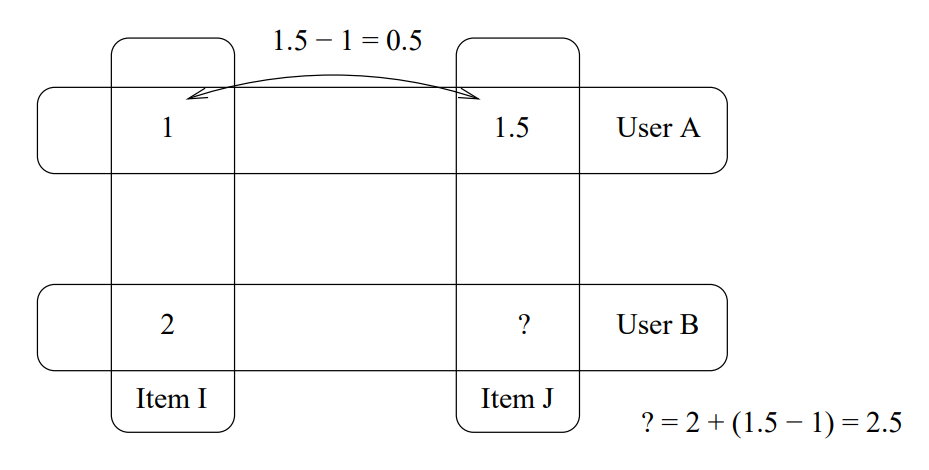
\includegraphics[keepaspectratio]{figures/algorithms/slope_one.PNG}
    \caption{Base dello schema Slope One: le valutazioni dello \textit{user} A di due \textit{item} e la valutazione  dello \textit{user} B di un \textit{item} comune vengono utilizzate per prevedere la valutazione sconosciuta dello \textit{user}.}
    \label{fig:slopeone}
\end{figure}

L'algoritmo soffre anche di diverse problematiche:
\begin{itemize}
    \item sparsità dei dati: le formule presentate prima sono approssimate considerando un dataset non sparso. Nel caso di matrici molto sparse l'algoritmo non sarà in grado di fare previsioni accurate
    \item scalabilità limitata su dataset molto grandi: la memoria necessaria per memorizzare le differenze medie dei \textit{rating} può aumentare rapidamente
    \item non tiene conto nè di personalizzazioni per \textit{user} 
    \item difficoltà a gestire grandi variazioni nelle valutazioni degli utenti
\end{itemize}

L'approccio può essere esteso a modelli ponderati e versioni più avanzate, come per esempio \emph{Weighted Slope One}, che pesa le differenze di \textit{rating} in base alla frequenza di coppie di \textit{item} valutati, e \emph{Regression-based Slope One}, che introduce funzioni non lineari per migliorare la precisione delle previsioni.

\subsubsection{Evaluation esplicita}\label{evaluation-esplicita}

\subsubsection{Algoritmi per Feedback Implicito}\label{algoritmi-per-feedback-implicito}

\subsubsection{ALS (Alternating Least Squares)}\label{als-alternating-least-squares}

\subsubsection{BPR (Bayesian Personalized Ranking)}\label{bpr-bayesian-personalized-ranking}

\subsubsection{LMF (Logistic Matrix Factorization)}\label{lmf-logistic-matrix-factorization}

\subsubsection{Evaluation implicita}\label{evaluation-implicita}

\subsubsection{Algoritmi per la Similarità Item-Item}\label{algoritmi-per-la-similarita-item-item}

\subsubsection{Algoritmi Ibridi}\label{algoritmi-ibridi}

\subsubsection{LightFM}\label{lightfm}

\subsubsection{Introduzione a Modelli di Deep Learning}\label{introduzione-a-modelli-di-deep-learning}
